\whiteBGstarBegin
\setcounter{section}{0}
\section{Động lượng - Định luật bảo toàn động lượng}
\begin{enumerate}[label=\bfseries Câu \arabic*:]
	
	\item \mkstar{1}
	
	\cauhoi{Một vật có khối lượng $m=\SI{1}{\kilogram}$ đang chuyển động với vận tốc $v=\SI{2}{\meter/\second}$. Tính động lượng của vật.
	}
	\loigiai
	{Động lượng của vật: $p=mv=\SI{2}{kg.m/s}$.
	}
	
	\item \mkstar{1}
	
	\cauhoi{Một vật có khối lượng $\SI{2}{\kilogram}$ và có động lượng $\SI{6}{kg.m/s}$. Vật đang chuyển động với vận tốc bao nhiêu?
	}
	\loigiai
	{Vận tốc của vật: $v=\dfrac{p}{m}=\SI{3}{m/s}$.
	}
	\item \mkstar{2}
	
	\cauhoi{Hai vật có khối lượng $m_1=\SI{1}{\kilogram}$, $m_2=\SI{3}{\kilogram}$ chuyển động với các vận tốc $v_1=\SI{3}{\meter/\second}$ và $v_2=\SI{1}{\meter/\second}$. Tìm tổng động lượng (phương, chiều và độ lớn) của hệ trong các trường hợp
		\begin{enumerate}[label=\alph*)]
			\item $\vec{v}_1$ và $\vec{v}_2$ cùng hướng.
			\item $\vec{v}_1$ và $\vec{v}_2$ cùng phương, ngược chiều.
			\item $\vec{v}_1$ và $\vec{v}_2$ vuông góc nhau.
			\item $\vec{v}_1$ và $\vec{v}_2$ hợp nhau một góc $120^\circ$.
		\end{enumerate}
	}
	\loigiai{
		
		\begin{enumerate}[label=\alph*)]
			\item $p=m_1v_1 + m_2v_2 = \SI{6}{kg.m/s}$.
			\item $p=|m_1v_1 - m_2v_2|=0$.
			\item $p=\sqrt{(m_1v_1)^2 + (m_2v_2)^2}=\xsi{3\sqrt2}{kg.m/s}$.
			\item $p=\sqrt{(m_1v_1)^2 + (m_2v_2)^2 + 2(m_1v_1)(m_2v_2)\cos 120^\circ} = \SI{3}{kg.m/s}$.
		\end{enumerate}
	}
\item \mkstar{2}

\cauhoi{Một quả bóng có khối lượng $m=\SI{300}{\gram}$ va chạm vào tường và nảy trở lại với cùng tốc độ. Vận tốc bóng trước va chạm là $\SI{5}{\meter/\second}$. Tìm độ biến thiên động lượng.
	
}
\loigiai{
	
	Độ biến thiên động lượng của quả bóng:
	$\Delta \vec p  = \vec p' - \vec p$.
	
	Vì $\vec p'$ và $\vec p$ cùng phương, ngược chiều nên $\Delta p = -2p = \SI{-3}{kg.m/s}$.
}
\item \mkstar{2}

\cauhoi{Một khẩu súng nằm ngang khối lượng $m_\text{s}=\SI{1000}{\kilogram}$, bắn một viên đạn khối lượng $m_\text{đ}=\SI{10}{\gram}$. Vận tốc viên đạn ra khỏi nòng súng là $\SI{600}{\meter/\second}$. Độ lớn vận tốc của súng sau khi bắn bằng là bao nhiêu?
	
}
\loigiai{
	
	Áp dụng định luật bảo toàn động lượng trước và sau khi bắn:
	$$m_1v_1 + m_2 v_2 = m_1v_1' + m_2 v_2' \Rightarrow 0 + 0 = \SI{1000}{kg} \cdot v_\text s + \SI{0.01}{kg} \cdot \SI{600}{m/s} \Rightarrow v_\text s = \SI{-6e-3}{m/s}$$
	
	Dấu $-$ chứng tỏ súng bị giật lùi.
}

\item \mkstar{2}

\cauhoi{Tên lửa có khối lượng vỏ là 10 tấn chuyển động với vận tốc $\SI{200}{\meter/\second}$ so với Trái Đất, 2 tấn khí phụt ra phía sau có vận tốc $\SI{500}{\meter/\second}$ so với Trái Đất. Xác định vận tốc của tên lửa so với Trái Đất sau khi khí phụt ra.
	
}
\loigiai{
	
	Áp dụng định luật bảo toàn động lượng trước và sau khi khí phụt ra:
	$$(m_1+m_2)v = m_1v_1 + m_2 v_2 \Rightarrow (\SI{10000}{kg} + \SI{2000}{kg}) \cdot \SI{200}{m/s} = \SI{10000}{kg} \cdot v_1 + \SI{2000}{kg} \cdot \SI{-500}{m/s}$$ $$\Rightarrow v_1  =\SI{340}{m/s}$$
}
	\item \mkstar{3}
	
	\cauhoi{Một xe có khối lượng 5 tấn bắt đầu hãm phanh chuyển động thẳng chậm dần đều dừng lại hẳn sau $\SI{20}{\second}$ kể từ lúc bắt đầu hãm phanh, trong thời gian đó xe chạy được $\SI{120}{\meter}$. Tính động lượng của xe lúc bắt đầu hãm phanh.
	}
	\loigiai
	{Vận tốc của xe lúc bắt đầu hãm phanh, giải hệ phương trình:
		
		$$\begin{cases}
			2aS=v^2 - v_0^2 \\
			v=at+v_0
		\end{cases}
		\Rightarrow
		\begin{cases}
			2a\cdot 120 =0 - v_0^2 \\
			0=a\cdot 20 + v_0
		\end{cases}
		\Rightarrow v_0 = \SI{12}{m/s}
		$$
		
		Động lượng của xe lúc bắt đầu hãm phanh: $p=mv_0=\SI{60000}{kg.m/s}$.
	}
	

	

	\item \mkstar{3}
	
	\cauhoi{Một vật có khối lượng $\SI{1}{\kilogram}$ rơi tự do xuống đất trong khoảng thời gian $\SI{0,5}{\second}$. Độ biến thiên động lượng của vật trong khoảng thời gian đó là bao nhiêu? Lấy $g=\SI{10}{\meter/\second^2}$.
		
	}
	\loigiai{
		
		Độ biến thiên vận tốc của vật:
		$\Delta v = gt = \SI{4.9}{m/s}$.
		
		Độ biến thiên động lượng của vật: $\Delta p = m\Delta v = \SI{4.9}{kg.m/s}$.
	}
	
		
	\item \mkstar{3}
	
	\cauhoi{Một quả bóng $\SI{2.5}{\kilogram}$ đập vào tường với vận tốc $\SI{8.5}{\meter/\second}$ và bị bật ngược trở lại với vận tốc $\SI{7.5}{m/s}$. Biết thời gian va chạm là $\SI{0.25}{\second}$. Tìm lực mà tường tác dụng lên quả bóng.
		
	}
	\loigiai{
		
		Độ biến thiên động lượng của quả bóng:
		$\Delta p = \SI{-40}{kg.m/s}$.
		
		Lưc mà tường tác dụng lên quả bóng: $F=\dfrac{\Delta p}{\Delta t} = \SI{-160}{N}$.
	}
	
	\item \mkstar{3}
	
	\cauhoi{Một toa xe khối lượng 10 tấn đang chuyển động trên đường ray nằm ngang với vận tốc không đổi $v=\SI{54}{\kilo\meter/\hour}$, người ta tác dụng lên toa xe một lực hãm theo phương ngang. Tính độ lớn trung bình của lực hãm nếu toa xe dừng lại sau
		\begin{enumerate}[label=\alph*)]
			\item 1 phút 40 giây.
			\item 10 giây.
		\end{enumerate}
		
	}
	\loigiai{
		
		\begin{enumerate}[label=\alph*)]
			\item $F=\dfrac{\Delta p}{\Delta t}=\SI{1500}{\newton}$.
			\item $F=\dfrac{\Delta p}{\Delta t}=\SI{15000}{\newton}$.
		\end{enumerate}
	}
	
	\item \mkstar{3}
	
	\cauhoi{Một viên đạn khối lượng $\SI{10}{\gram}$ đang bay với vận tốc $\SI{600}{\meter/\second}$ thì gặp một bức tường. Đạn xuyên qua tường trong thời gian $\dfrac{1}{100}\,\text{s}$. Sau khi xuyên qua tường, vận tốc của đạn còn $\SI{200}{\meter/\second}$. Tính lực cản của tường tác dụng lên viên đạn.
		
	}
	\loigiai{
		Độ biến thiên động lượng của viên đạn:
		$\Delta p = m\Delta v = \SI{4}{kg.m/s}$.
		
		Lực cản của tường tác dụng lên viên đạn: $F=\dfrac{\Delta p}{\Delta t} = \SI{400}{N}$.
	}
	
	
	
	\item \mkstar{3}
	
	\cauhoi{Vật $m_1$ chuyển động với vận tốc $\SI{6}{\meter/\second}$ đến va chạm với vật $m_2$ chuyển động ngược chiều với vận tốc $\SI{2}{\meter/\second}$. Sau va chạm, hai vật bật ngược trở lại với vận tốc $\SI{4}{\meter/\second}$. Tính khối lượng của hai vật biết $m_1+m_2=\SI{ 1,5}{\kilogram}$.
		
	}
	\loigiai{
		
		Ta có $m_1+m_2=\SI{ 1,5}{\kilogram}$.
		
		Áp dụng định luật bảo toàn động lượng trong va chạm đàn hồi:
		$$m_1v_1 + m_2 v_2 = m_1v_1' + m_2 v_2' \Rightarrow m_1\cdot\SI{6}{m/s} + m_2 \cdot \SI{-2}{m/s} = m_1 \cdot \SI{-4}{m/s} + m_2 \cdot \SI{4}{m/s}.$$
		
		Giải hệ 2 phương trình trên, thu được
		$\begin{cases}
			m_1=\SI{0,5625}{\kilogram}\\
			m_2=\SI{0,9375}{\kilogram}.
		\end{cases}$
	}
	
	\item \mkstar{3}
	
	\cauhoi{Vật $\SI{200}{\gram}$ chuyển động với vận tốc $\SI{6}{\meter/\second}$ đến va chạm với vật $\SI{50}{\gram}$ chuyển động với vận tốc $\SI{4}{\meter/\second}$. Sau va chạm vật $\SI{200}{\gram}$ giữ nguyên hướng và chuyển động với vận tốc bằng nửa vận tốc ban đầu. Tính vận tốc của vật còn lại trong các trường hợp sau:
		\begin{enumerate}[label=\alph*)]
			\item Trước va chạm hai vật chuyển động cùng chiều.
			\item Trước va chạm hai vật chuyển động ngược chiều.
		\end{enumerate}
		
	}
	\loigiai{
		
		\begin{enumerate}[label=\alph*)]
			\item Trước va chạm hai vật chuyển động cùng chiều.
			
			Áp dụng định luật bảo toàn động lượng trong va chạm đàn hồi:
			$$m_1v_1 + m_2 v_2 = m_1v_1' + m_2 v_2' \Rightarrow \SI{0.2}{kg} \cdot \SI{6}{m/s} + \SI{0.05}{kg} \cdot \SI{4}{m/s} = \SI{0.2}{kg} \cdot \SI{3}{m/s} + \SI{0.05}{kg} \cdot v_2'$$ $$\Rightarrow v_2'=\SI{16}{m/s}$$
			
			\item Trước va chạm hai vật chuyển động ngược chiều.
			
			Áp dụng định luật bảo toàn động lượng trong va chạm đàn hồi:
			$$m_1v_1 + m_2 v_2 = m_1v_1' + m_2 v_2' \Rightarrow \SI{0.2}{kg} \cdot \SI{6}{m/s} + \SI{0.05}{kg} \cdot \SI{-4}{m/s} = \SI{0.2}{kg} \cdot \SI{3}{m/s} + \SI{0.05}{kg} \cdot v_2'$$ $$\Rightarrow v_2'=\SI{8}{m/s}$$
		\end{enumerate}
	}
	
	
\item \mkstar{4}

\cauhoi{Từ độ cao $h=\SI{80}{\meter}$, ở thời điểm $t_0=0$ một vật $\SI{200}{\gram}$ được ném ngang với vận tốc ban đầu $v_0=10\sqrt{3}\,\text{m/s}$, gia tốc trọng trường $g=\SI{10}{\meter/\second^2}$. Tìm động lượng của vật ở thời điểm $t=\SI{1}{\second}$.
}
\loigiai
{Tại thời điểm $t=\SI{1}{\second}$, vận tốc theo các phương $x$ và $y$ là
	$$
	\begin{cases}
		v_x=v_0=10\sqrt{3}\,\text{m/s} \\
		v_y=gt=10\,\text{m/s}
	\end{cases}
	$$
	
	Vận tốc của vật tại thời điểm $t=\SI{1}{\second}$: $v=\sqrt{v_x^2 + v_y^2} = \SI{20}{m/s}$.
	
	Động lượng của vật tại thời điểm $t=\SI{1}{\second}$: $p=mv=\SI{4}{kg.m/s}$.
	
}
\item \mkstar{4}

\cauhoi{Xác định độ biến thiên động lượng của một vật có khối lượng $\SI{4}{\kilogram}$ sau khoảng thời gian 6 giây. Biết rằng vật chuyển động trên đường thẳng và có phương trình chuyển động là $x=t^2-6t+3$.
	
}
\loigiai{
	
	Gia tốc của vật: $a=\SI{2}{m/s^2}$.
	
	Vận tốc ban đầu của vật: $v_0 = \SI{-6}{m/s}$.
	
	Độ biến thiên vận tốc của vật:
	$\Delta v = v-v_0 = v_0+at-v_0=at = \SI{12}{m/s}$.
	
	Độ biến thiên động lượng của vật: $\Delta p = m\Delta v = \SI{48}{kg.m/s}$.
}
\end{enumerate}

\section{Công và công suất}
\begin{enumerate}[label=\bfseries Câu \arabic*:]
	
			\item \mkstar{2}
	
	\cauhoi{
		Một vật có khối lượng $m=\SI{500}{\gram}$ trượt từ đỉnh B đến chân C của một mặt phẳng nghiêng có chiều dài $l=\text{BC}=\SI{2}{\meter}$, góc nghiêng $\beta$; $g=\SI{10}{\meter/\second^2}$. Công của trọng lực thực hiện khi vật di chuyển từ B đến C bằng $\SI{4}{\joule}$.
		\begin{center}
			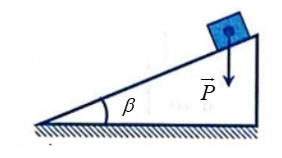
\includegraphics[scale=0.9]{../figs/VN10-PH-30-P-022-1-H1.jpg}
		\end{center}
		Giá trị của $\beta$ xấp xỉ bằng
		\begin{mcq}(4)
			\item $30^\circ$.
			\item $31^\circ$.
			\item $51^\circ$.
			\item $24^\circ$.
		\end{mcq}
		
	}
	
	\loigiai{
		\textbf{Đáp án: D.}
		
		Công của trọng lực:
		$$A=mgh = mg l \sin \beta \Rightarrow \sin \beta = 0,4 \Rightarrow \beta \approx 24^\circ$$
	}
	\item \mkstar{3}
	
	\cauhoi{
		Một vật khối lượng $m=\SI{10}{\kilogram}$ được kéo chuyển động thẳng nhanh dần dều trên sàn nhẵn không ma sát bằng một lực $F=\SI{5}{\newton}$ theo phương ngang từ trạng thái nghỉ. Trong thời gian 4 giây tính từ lúc bắt đầu chuyển động công suất trung bình của lực $F$ bằng
		\begin{mcq}(4)
			\item $\SI{10}{\watt}$.
			\item $\SI{8}{\watt}$.
			\item $\SI{5}{\watt}$.
			\item $\SI{4}{\watt}$.
		\end{mcq}
		
	}
	
	\loigiai{
		\textbf{Đáp án: D.}
		
		Gia tốc vật thu được:
		$$a=\dfrac{F}{m} = \SI{0.5}{m/s^2}$$
		
		Quãng đường vật đi được:
		$$s=\dfrac{1}{2}at^2 = \SI{4}{m}$$
		
		Công của lực $F$:
		$$A=Fs= \SI{20}{J}$$
		
		Công suất trung bình của lực $F$:
		$$\calP = \dfrac{A}{t} = \SI{5}{W}$$
	}
	\item \mkstar{4}
	
	\cauhoi{
		Một người kéo một vật có $m=\SI{8}{\kilogram}$ trượt trên mặt phẳng ngang có hệ số ma sát $\mu=0,2$ bằng một sợi dây có phương hợp một góc $60^\circ$ so với phương nằm ngang. Lực tác dụng lên dây bằng $\vec{F}_\text{k}$, vật trượt không vận tốc đầu với $a=\SI{1}{\meter/\second^2}$. Công của lực kéo trong thời gian 4 giây kể từ khi bắt đầu chuyển động là (lấy $g=\SI{10}{m/s^2}$)
		\begin{mcq}(4)
			\item $\SI{162,5}{\joule}$.
			\item $\SI{140,7}{\joule}$.
			\item $\SI{142,6}{\joule}$.
			\item $\SI{126,7}{\joule}$.
		\end{mcq}
		
	}
	
	\loigiai{
		\textbf{Đáp án: C.}
		
		Quãng đường vật đi được trong 4 giây:
		$$s=\dfrac{1}{2}at^2 = \SI{8}{m}$$
		
		Áp dụng định luật II Newton theo phương thẳng đứng:
		$$F_y + N =P\Rightarrow N = mg -F_y = mg - F \sin \alpha$$
		
		Áp dụng định luật II Newton theo phương ngang:
		$$F_x - F_\text{ms} = ma \Rightarrow F \cos \alpha - F_\text{ms} = ma \Rightarrow F \cos \alpha -  \mu (mg - F \sin \alpha) = ma$$
		
		Tìm được độ lớn lực $F$:
		$$F=\SI{35,65}{N}$$
		
		Công của lực kéo:
		$$A=Fs\cos \alpha  = \SI{142.6}{J}$$
	}
	
	\item \mkstar{4}
	
	\cauhoi{
		Một vật có khối lượng $m=\SI{3}{\kilogram}$ được kéo lên trên mặt phẳng nghiêng một góc $30^\circ$ so với phương ngang bởi một lực không đổi $F=\SI{70}{\newton}$ dọc theo mặt phẳng nghiêng. Biết hệ số ma sát là 0,05, lấy $g=\SI{10}{\meter/\second^2}$. Tổng công của tất cả các lực tác dụng lên vật là $\SI{215}{\joule}$.
		\begin{center}
			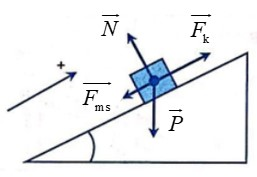
\includegraphics[scale=0.9]{../figs/VN10-PH-30-P-022-1-H2.jpg}
		\end{center}
		Quãng đường tương ứng vật đã di chuyển bằng
		\begin{mcq}(4)
			\item $\SI{1}{\meter}$.
			\item $\SI{2}{\meter}$.
			\item $\SI{4}{\meter}$.
			\item $\SI{6}{\meter}$.
		\end{mcq}
		
	}
	
	\loigiai{
		\textbf{Đáp án: C.}
		
		Phản lực $\vec N$ vuông góc với mặt nghiêng nên công bằng $0$.
		
		Công của trọng lực là công cản: 
		$$A_1=-mgh = -mgs\sin \alpha$$
		
		Công của lực kéo là công phát động:
		$$A_2 = Fs$$
		
		Công của lực ma sát là công cản:
		$$A_3= -\mu N s = -\mu mg \cos \alpha s$$
		
		Tổng công các lực:
		$$A=A_1+A_2+A_3 = \SI{215}{J} \Rightarrow s  =\SI{4}{m}$$
	}

		\item \mkstar{2}
		
		\cauhoi{
			Một ô tô có khối lượng 1,2 tấn chuyển động đều trên mặt đường nằm ngang với vận tốc $v=\SI{36}{\kilo\meter/\hour}$. Hỏi phải thực hiện một công là bao nhiêu để hãm xe dừng lại?
		}
		
		\loigiai{
			Áp dụng công thức:
			$$2as = v^2 - v_0^2 \Rightarrow as=\dfrac{0-10^2}{2}$$
			
			Công của lực thực hiện để xe dừng lại:
			$$A=Fs = mas =\SI{-60000}{J} $$
		}

\item \mkstar{3}

\cauhoi{
	Một xe tải có khối lượng 2,5 tấn bắt đầu chuyển động thẳng nhanh dần đều, sau khi đi được quãng đường $\SI{144}{\meter}$ thì xe đạt vận tốc $\SI{12}{\meter/\second}$. Biết hệ số ma sát giữa xe và mặt đường là $\mu=0,04$. Lấy $g= \SI{10}{\meter/\second^2}$.
	\begin{enumerate}[label=\alph*)]
		\item Tính tổng công của các lực tác dụng lên xe trên quãng đường $\SI{144}{\meter}$ đầu tiên.
		\item Tính công suất của lực do động cơ xe hoạt động ở quãng đường nói trên.
		\item Tính hiệu suất hoạt động của động cơ xe.
	\end{enumerate}
}

\loigiai{		
	\begin{enumerate}[label=\alph*)]
		\item Tính tổng công của các lực tác dụng lên xe trên quãng đường $\SI{144}{\meter}$ đầu tiên.
		
		Gia tốc mà xe thu được:
		$$2as = v^2 - v_0^2 \Rightarrow a = \SI{0.5}{m/s^2}$$
		
		Tổng hợp lực tác dụng lên xe:
		$$\Sigma F = ma = \SI{1250}{N}$$
		
		Tổng công các lực tác dụng lên xe:
		$$A=\Sigma F s = \SI{180000}{J}$$
		\item Tính công suất của lực do động cơ xe hoạt động ở quãng đường nói trên.
		
		Công của lực phát động của động cơ xe:
		$$A_F = A-A_\text{ms} = A- (-\mu mg s) = \SI{324000}{J}$$
		
		Thời gian xe chuyển động:
		$$v=at+v_0 \Rightarrow t = \SI{24}{s}$$
		
		Công suất của động cơ:
		$$\calP = \dfrac{A_F}{t} = \SI{13500}{W}$$
		\item Tính hiệu suất hoạt động của động cơ xe.
		
		$$H=\dfrac{A}{A_F} = \SI{55.56}{\percent}$$
	\end{enumerate}
}
\end{enumerate}

\section{Động năng}
\begin{enumerate}[label=\bfseries Câu \arabic*:]
	
		\item \mkstar{1}
	
	\cauhoi{
		Nhận định nào sau đây về động năng là không đúng?
		\begin{mcq}(1)
			\item Động năng là đại lượng vô hướng và luôn dương.
			\item Động năng có tính tương đối, phụ thuộc hệ quy chiếu.
			\item Động năng tỷ lệ thuận với khối lượng và vận tốc của vật.
			\item Động năng là năng lượng của vật đang chuyển động.
		\end{mcq}
	}
	
	\loigiai{
		\textbf{Đáp án: C.}
		
		Động năng tỷ lệ thuận với khối lượng và bình phương vận tốc của vật.
	}
	
	\item \mkstar{2}
	
	\cauhoi{
		Một ô tô có khối lượng 1,5 tấn đang chuyển động thẳng đều trong 2 giờ xe đi được quãng đường $\SI{72}{\kilo\meter}$. Động năng của ô tô này bằng
		\begin{mcq}(4)
			\item $\SI{972}{\joule}$.
			\item $\SI{150}{\kilo\joule}$.
			\item $\SI{75}{\kilo\joule}$.
			\item $\SI{972}{\kilo\joule}$.
		\end{mcq}
	}
	
	\loigiai{
		\textbf{Đáp án: C.}
		
		Vận tốc của ô tô:
		$$v=\dfrac{s}{t} = \SI{10}{m/s}$$
		
		Động năng của ô tô:
		$$W_\text{đ} = \dfrac{1}{2} mv^2 = \SI{75}{kJ}$$
	}
	\item \mkstar{2}
	
	\cauhoi{
		Một ô tô có khối lượng 4 tấn đang chuyển động với vận tốc $\SI{36}{\kilo\meter/\hour}$ thì hãm phanh, sau một thời gian vận tốc giảm còn $\SI{18}{\kilo\meter/\hour}$. Độ biến thiên của động năng của ô tô là
		\begin{mcq}(4)
			\item $\SI{150}{\kilo\joule}$.
			\item $\SI{-150}{\kilo\joule}$.
			\item $\SI{-75}{\kilo\joule}$.
			\item $\SI{75}{\kilo\joule}$.
		\end{mcq}
	}
	
	\loigiai{
		\textbf{Đáp án: B.}
		
		Độ biến thiên động năng:
		$$\Delta W_\text{đ} = \dfrac{1}{2} m (v^2 - v_0^2) = \SI{-150}{kJ}$$
	}
	\item \mkstar{3}
	
	\cauhoi{
		Một hòn đá có khối lượng $m=\SI{200}{\gram}$ rơi tự do không vận tốc đầu từ một điểm cách mặt đất $\SI{45}{\meter}$, tại nơi có gia tốc trọng trường $g= \SI{10}{\meter/\second^2}$. Động năng của hòn đá ngay trước khi chạm đất là
		\begin{mcq}(4)
			\item $\SI{45}{\joule}$.
			\item $\SI{90}{\joule}$.
			\item $\SI{180}{\joule}$.
			\item $\SI{900}{\joule}$.
		\end{mcq}
	}
	
	\loigiai{
		\textbf{Đáp án: B.}
		
		Thời gian rơi:
		$$h=\dfrac{1}{2}gt^2 \Rightarrow t = \SI{3}{s}$$
		
		Vận tốc của hòn đá ngay trước khi chạm đất:
		$$v=gt= \SI{30}{m/s}$$
		
		Động năng hòn đá ngay trước khi chạm đất:
		$$W_\text{đ} = \dfrac{1}{2} mv^2 = \SI{90}{J}$$
	}
\item \mkstar{3}

\cauhoi{
	Một ô tô có khối lượng $\SI{1600}{\kilogram}$ đang chạy với tốc độ $\SI{54}{\kilo\meter/\hour}$ thì người lái xe nhìn thấy một vật cản trước mặt cách khoảng $\SI{10}{\meter}$. Người đó tắt máy và hãm phanh khẩn cấp với lực hãm không đổi là $\SI{2e4}{\newton}$. Xe dừng lại cách vật cản một khoảng bằng
	\begin{mcq}(4)
		\item $\SI{1,2}{\meter}$.
		\item $\SI{1,0}{\meter}$.
		\item $\SI{1,4}{\meter}$.
		\item $\SI{1,5}{\meter}$.
	\end{mcq}
}

\loigiai{
	\textbf{Đáp án: B.}
	
	Quãng đường xe chạy được cho đến khi dừng hẳn theo lý thuyết định lý động năng là
	$$-F_\text{h}s = 0 - \dfrac{1}{2}mv^2 \Rightarrow s = \SI{9}{m}$$
	
	Vậy xe dừng lại cách vật cản một khoảng bằng $\SI{10}{m}-\SI{9}{m}=\SI{1}{m}$.
}
\item \mkstar{3}

\cauhoi{
	Trung tâm bồi dưỡng kiến thức Hà Nội tổ chức một cuộc thi cho các học viên chạy. Có một học viên có trọng lượng $\SI{700}{\newton}$ chạy đều hết quãng đường $\SI{600}{\meter}$ trong $\SI{50}{\second}$. Tìm động năng của học viên đó. Lấy $g= \SI{10}{\meter/\second^2}$.
}

\loigiai{
	Khối lượng của học viên:
	$$m=\dfrac{P}{g} = \SI{70}{kg}$$
	
	Vận tốc chạy của học viên:
	$$v=\dfrac{s}{t} = \SI{12}{m/s}$$
	
	Động năng của học viên:
	$$W_\text{đ} = \dfrac{1}{2}mv^2 = \SI{5040}{J}$$
}

\item \mkstar{2}

\cauhoi{
	Vận động viên Hoàng Xuân Vinh bắn một viên đạn có khối lượng $\SI{100}{\gram}$ bay ngang với vận tốc $\SI{300}{\meter/\second}$ xuyên qua tấm bia bằng gỗ dày $\SI{5}{\centi\meter}$. Sau khi xuyên qua bia gỗ thì đạn có vận tốc $\SI{100}{\meter/\second}$. Tính lực cản của tấm bia gỗ tác dụng lên viên đạn.
}
\loigiai{
	
	Áp dụng định lý động năng:
	$$-F_\text{cản}s = \dfrac{1}{2}m(v^2-v_0^2) \Rightarrow F_\text{cản} = \SI{80000}{N}$$
}

\item \mkstar{3}

\cauhoi{
	Một vật có khối lượng $\SI{2}{\kilogram}$ trượt qua A với vận tốc $\SI{2}{\meter/\second}$ xuống dốc nghiêng AB dài $\SI{2}{\meter}$, cao $\SI{1}{\meter}$. Biết hệ số ma sát giữa vật và mặt phẳng nghiêng là $\mu=\dfrac{1}{\sqrt{3}}$. Lấy $g= \SI{10}{\meter/\second^2}$.
	\begin{enumerate}[label=\alph*)]
		\item Xác định công của trọng lực, công của lực ma sát thực hiện khi vật chuyển dời từ dinh dốc đến chân dốc.
		\item Xác định vận tốc của vật tại chân dốc B.
		\item Tại chân dốc B vật tiếp tục chuyển dộng trên mặt phẳng nằm ngang BC dài $\SI{2}{\meter}$ thì dừng lại. Xác định hệ số ma sát trên đoạn dường BC này.
	\end{enumerate}
}
\loigiai{
	
	\begin{enumerate}[label=\alph*)]
		\item Xác định công của trọng lực, công của lực ma sát thực hiện khi vật chuyển dời từ dinh dốc đến chân dốc.
		
		Góc nghiêng của mặt phẳng nghiêng:
		$$\sin \alpha = \dfrac{h}{l} = \dfrac{1}{2} \Rightarrow \alpha = 30^\circ $$
		
		Công của trọng lực:
		$$A_1 = mgh  = \SI{20}{J}$$
		
		Độ lớn lực ma sát:
		$$F_\text{ms} = \mu N = \mu mg\cos \alpha = \SI{10}{N}$$
		
		Công của lực ma sát:
		$$A_2=-F_\text{ms} l = \SI{-20}{J}$$
		\item Xác định vận tốc của vật tại chân dốc B.
		
		Áp dụng định lý động năng:
		$$A_1+A_2 = \dfrac{1}{2}mv_\text{B}^2 -\dfrac{1}{2}mv_\text{A}^2 =0\Rightarrow v_\text{B} =v_\text A =  \SI{2}{m/s}$$
		\item Tại chân dốc B vật tiếp tục chuyển dộng trên mặt phẳng nằm ngang BC dài $\SI{2}{\meter}$ thì dừng lại. Xác định hệ số ma sát trên đoạn dường BC này.
		
		Áp dụng định lý động năng:
		$$ -\mu_2 mg s_2 = 0-\dfrac{1}{2}mv_\text B^2 \Rightarrow \mu_2 = \SI{0.1}{}$$
	\end{enumerate}
}

\item \mkstar{3}

\cauhoi{
	Một xe có khối lượng 2 tấn chuyên động trên đoạn AB nằm ngang với vận tốc không đổi $\SI{7,2}{\kilo\meter/\hour}$, lấy $g= \SI{10}{\meter/\second^2}$.
	\begin{enumerate}[label=\alph*)]
		\item Đến điểm B thì xe tắt máy và xuống dốc BC nghiêng góc $30^\circ$ so với phương ngang, bỏ qua ma sát. Biết vận tốc tại chân C là $\SI{72}{\kilo\meter/\hour}$. Tìm chiều dài dốc BC.
		\item Tại C xe tiếp tục chuyển động trên đoạn đường nằm ngang CD và đi thêm được $\SI{200}{\meter}$ thì dừng lại. Tìm hệ số ma sát trên đoạn CD.
	\end{enumerate}
}
\loigiai{
	
	\begin{enumerate}[label=\alph*)]
		\item Đến điểm B thì xe tắt máy và xuống dốc BC nghiêng góc $30^\circ$ so với phương ngang, bỏ qua ma sát. Biết vận tốc tại chân C là $\SI{72}{\kilo\meter/\hour}$. Tìm chiều dài dốc BC.
		
		Bỏ qua ma sát, áp dụng định lý động năng:
		$$A_P=\dfrac{1}{2}mv_\text{C}^2 - \dfrac{1}{2}mv_\text{B}^2 \Rightarrow mgl \sin \alpha = \dfrac{1}{2} mv_\text{C}^2 - \dfrac{1}{2}mv_\text{B}^2 \Rightarrow l = \SI{39.6}{m}$$
		\item Tại C xe tiếp tục chuyên động trên đoạn đường nằm ngang CD và đi thêm được $\SI{200}{\meter}$ thì dừng lại. Tìm hệ số ma sát trên đoạn CD.
		
		Áp dụng định lý động năng:
		$$A_\text{ms} = 0- \dfrac{1}{2}mv_\text{C}^2 \Rightarrow -\mu mgs = - \dfrac{1}{2}mv_\text{C}^2 \Rightarrow \mu = \SI{0.1}{}$$
	\end{enumerate}
}

\item \mkstar{4}

\cauhoi{
	Một ô tô có khối lượng 2 tấn đang chuyển dộng trên đường thẳng nằm ngang AB dài $\SI{100}{\meter}$, khi qua A vận tốc ô tô là $\SI{10}{\meter/\second}$ và đến B vận tốc của ô tô là $\SI{20}{\meter/\second}$. Biết độ lớn của lực kéo là $\SI{4000}{\newton}$.
	\begin{enumerate}[label=\alph*)]
		\item Tìm hệ số ma sát $\mu_1$ trên đoạn đường AB.
		\item Đến B thì động cơ tắt máy và lên dốc BC dài $\SI{40}{\meter}$ nghiêng $30^\circ$ so với mặt phẳng ngang. Hệ số ma sát trên mặt dốc là $\mu_2=\dfrac{1}{5\sqrt{3}}$. Hỏi xe có lên đến đỉnh dốc C không?
		\item Nếu đến B với vận tốc trên, muốn xe lên dốc và dừng lại tại C thì phải tác dụng liên tục lên xe một lực có độ lớn bao nhiêu?
	\end{enumerate}
}
\loigiai{
	
	\begin{enumerate}[label=\alph*)]
		\item Tìm hệ số ma sát $\mu_1$ trên đoạn đường AB.
		
		Áp dụng định lý động năng:
		$$-\mu_1 mg s_1 + Fs_1 = \dfrac{1}{2}mv_\text{B}^2 - \dfrac{1}{2}mv_\text{A}^2 \Rightarrow \mu_1 = \SI{0.05}{}$$
		\item Đến B thì động cơ tắt máy và lên dốc BC dài $\SI{40}{\meter}$ nghiêng $30^\circ$ so với mặt phẳng ngang. Hệ số ma sát trên mặt dốc là $\mu_2=\dfrac{1}{5\sqrt{3}}$. Hỏi xe có lên đến đỉnh dốc C không?
		
		Áp dụng định lý động năng từ B đến khi xe dừng lại:
		$$A_\text{ms2}+A_{P2} = 0 - \dfrac{1}{2}mv_\text{B}^2 \Rightarrow -\mu_2 mg \cos \alpha s_2 - mgs_2 \sin \alpha = 0 - \dfrac{1}{2}mv_\text{B}^2 \Rightarrow s_2 = \SI{33.33}{m}$$
		
		Vậy quãng đường tối đa xe lên được là $\SI{33.33}{m}$, mà dốc dài $\SI{40}{m}$ nên xe không lên được đến đỉnh dốc.
		\item Nếu đến B với vận tốc trên, muốn xe lên dốc và dừng lại tại C thì phải tác dụng liên tục lên xe một lực có độ lớn bao nhiêu?
		
		Để xe lên được đến C thì $s_3=\SI{40}{m}$, khi đó:
		$$A_\text{ms3}+A_{P3}+A_F = 0 - \dfrac{1}{2}mv_\text{B}^2 \Rightarrow -\mu_2 mg \cos \alpha s_3 - mgs_3 \sin \alpha +Fs_3= 0 - \dfrac{1}{2}mv_\text{B}^2 \Rightarrow F = \SI{1}{N}$$
	\end{enumerate}
}
\end{enumerate}

\section{Thế năng}
\begin{enumerate}[label=\bfseries Câu \arabic*:]
	
\item \mkstar{1}

\cauhoi{
	Biểu thức nào sau đây không phải biểu thức của thế năng?
	\begin{mcq}(2)
		\item $W_\text{t}=mgh$.
		\item $W_\text t=mg(z_2-z_1)$.
		\item $W_\text t=Ph$.
		\item $W_\text t=\dfrac{1}{2}mgh$.
	\end{mcq}
	
}

\loigiai{
	\textbf{Đáp án: D.}
	
	$\dfrac{1}{2}mgh$ không phải là biểu thức của thế năng.
}
\item \mkstar{1}

\cauhoi{
	Một vật nằm yên (trong hệ quy chiếu đứng yên) có thể có
	\begin{mcq}(4)
		\item thế năng.
		\item vận tốc.
		\item động năng.
		\item động lượng.
	\end{mcq}
	
}

\loigiai{
	\textbf{Đáp án: A.}
	
	Một vật nằm yên không thể có động lượng, động năng, vận tốc, nhưng có thể có thế năng.
}
\item \mkstar{1}

\cauhoi{
	Thế năng của vật nặng $\SI{2}{\kilogram}$ ở đáy một giếng sâu $\SI{10}{\meter}$ so với mặt đất tại nơi có gia tốc $g= \SI{10}{\meter/\second^2}$ là bao nhiêu?
	\begin{mcq}(4)
		\item $\SI{-100}{\joule}$.
		\item $\SI{100}{\joule}$.
		\item $\SI{200}{\joule}$.
		\item $\SI{-200}{\joule}$. 
	\end{mcq}
}

\loigiai{\textbf{Đáp án: D.}
	
	Thế năng trọng trường:
	$$W_\text t= mgz = \SI{-200}{J}$$
	
}
\item \mkstar{1}

\cauhoi{
	Một lò xo bị nén $\SI{5}{\centi\meter}$. Biết độ cứng lò xo $k=\SI{100}{\newton/\meter}$, thế năng của lò xo là
	\begin{mcq}(4)
		\item $\SI{0,125}{\joule}$.
		\item $\SI{0,25}{\joule}$.
		\item $\SI{125}{\joule}$.
		\item $\SI{250}{\joule}$.
	\end{mcq}
	
}

\loigiai{
	\textbf{Đáp án: A.}
	
	Thế năng đàn hồi của lò xo:
	$$W_\text t= \dfrac{1}{2} k (\Delta l)^2 = \SI{0,125}{\joule}$$
}
\item \mkstar{1}

\cauhoi{
	Một lò xo có độ cứng $\SI{100}{\newton/\meter}$, một đầu cố định, đầu kia gắn với vật nhỏ. Khi lò xo bị nén $\SI{4}{\centi\meter}$ thì thế năng đàn hồi của hệ là
	\begin{mcq}(4)
		\item $\SI{800}{\joule}$.
		\item $\SI{0,08}{\joule}$.
		\item $\SI{8}{\joule}$.
		\item $\SI{80}{\joule}$. 
	\end{mcq}
	
}

\loigiai{
	\textbf{Đáp án: A.}
	
	Thế năng đàn hồi của lò xo:
	$$W_\text t= \dfrac{1}{2} k (\Delta l)^2 = \SI{0.08}{\joule}$$
}

\item \mkstar{2}

\cauhoi{
	Một người có khối lượng $\SI{60}{\kilogram}$ đứng trên mặt đất và cạnh một cái giếng nước, lấy $g=$$\SI{10}{\meter/\second^2}$.
	\begin{enumerate}[label=\alph*)]
		\item Tính thế năng của người tại A cách mặt đất $\SI{3}{\meter}$ về phía trên và tại đáy giếng cách mặt đất $\SI{5}{\meter}$ với gốc thế năng tại mặt đất.
		\item Nếu lấy mốc thế năng tại đáy giếng, hãy tính lại kết quả câu trên.
	\end{enumerate}
}

\loigiai{
	
	\begin{enumerate}[label=\alph*)]
		
		\item Tính thế năng của người tại A cách mặt đất $\SI{3}{\meter}$ về phía trên và tại đáy giếng cách mặt đất $\SI{5}{\meter}$ với gốc thế năng tại mặt đất.
		
		Thế năng của người tại A cách mặt đất $\SI{3}{\meter}$ về phía trên (với $h_1=\SI{3}{m})$:
		
		$$W_\text t = mgh_1 = \SI{1800}{J}$$
		
		Thế năng của người tại đáy giếng cách mặt đất $\SI{5}{\meter}$ (với $h_2=\SI{-5}{m}$):
		$$W_\text t = mgh_2 = \SI{-3000}{J}$$
		
		\item Nếu lấy mốc thể năng tại đáy giếng, hãy tính lại kết quả câu trên.
		
		Thế năng của người tại A cách mặt đất $\SI{3}{\meter}$ về phía trên (với $h_3=\SI{8}{m}$):
		$$W_\text t = mgh_3 = \SI{4800}{J}$$
		
		Thế năng của người tại đáy giếng cách mặt đất $\SI{5}{\meter}$ (với $h_4=0$):
		$$W_\text t = mgh_4 = \SI{0}{J}$$
	\end{enumerate}
}



\item \mkstar{2}

\cauhoi{
	Cho một lò xo nằm ngang có độ cứng $k=\SI{100}{\newton/\meter}$. Công của lực đàn hồi thực hiện khi lò xo bị kéo dãn từ $\SI{2}{\centi\meter}$ đến $\SI{4}{\centi\meter}$ là bao nhiêu?	
	
}
\loigiai{
	
	Độ giảm thế năng bằng công của lực thế:
	$$A = W_\text{t 1} - W_\text{t 2} = \dfrac{1}{2} k (\Delta l_1 ^2 - \Delta l_2^2) = \SI{-0.06}{J}$$
}
\item \mkstar{3}

\cauhoi{
	Một học sinh của trung tâm bồi dưỡng kiến thức Hà Nội thả một vật rơi tự do có khối lượng $\SI{500}{\gram}$ từ độ cao $\SI{45}{\meter}$ so với mặt đất, bỏ qua ma sát với không khí, Tính thế năng của vật tại giây thứ hai so với mặt đất. Cho $g= \SI{10}{\meter/\second^2}$.
}

\loigiai{
	Độ cao của vật tại giây thứ hai so với mặt đất:
	$$h_2 = h - \dfrac{1}{2}gt^2 = \SI{25}{m}$$
	
	Thế năng của vật tại giây thứ hai so với mặt đất (gốc thế năng tại mặt đất):
	$$W_\text t = mgh_2 = \SI{125}{J}$$
}

\end{enumerate}

\section{Cơ năng}
\begin{enumerate}[label=\bfseries Câu \arabic*:]
	
	\item \mkstar{2}
	
	\cauhoi{
		Một học sinh ném một vật có khối lượng $\SI{200}{\gram}$ thẳng đứng lên cao với vận tốc ban đầu $\SI{8}{\meter/\second}$ từ độ cao $\SI{8}{\meter}$ so với mặt đất. Lấy $g= \SI{10}{\meter/\second^2}$. Xác định vận tốc của vật khi $W_\text{đ}=2W_\text{t}$.
	}
	
	\loigiai{
		Chọn gốc thế năng tại mặt đất.
		
		Cơ năng ban đầu:
		$$W_1 = W_\text{đ 1} + W_\text{t 1}  = \SI{22.4}{J}$$
		
		Khi $W_\text{đ 2} = 2 W_\text{t 2}$ thì $W_2 = \dfrac{3}{2} W_\text{đ 2}$. Áp dụng bảo toàn cơ năng:
		$$W_1 = W_2 \Rightarrow W_1 = \dfrac{3}{2}\cdot \dfrac{1}{2}mv_2^2 \Rightarrow v_2 = \SI{12.22}{m/s} $$
		
	}
	
	\item \mkstar{2}
	
	\cauhoi{
		Cho một vật có khối lượng $m$. Truyền cho vật một cơ năng là $\SI{37,5}{\joule}$. Khi vật chuyển động ở độ cao $\SI{3}{\meter}$ vật có $W_\text{đ}=\dfrac{3}{2}W_\text{t}$. Xác định khối lượng của vật và vận tốc của vật ở độ cao đó. Lấy $g= \SI{10}{\meter/\second^2}$.
		
	}
	
	\loigiai{
		
		Khi vật có $W_\text{đ 2} = \dfrac{3}{2} W_\text{t 2}$ thì $W_2 = \dfrac{5}{2} W_\text{t 2}$. Áp dụng bảo toàn cơ năng (với $z_2=\SI{3}{m}$):
		$$W_1 = W_2 \Rightarrow \SI{37.5}{J} = \dfrac{5}{2} mgz_2 \Rightarrow m =\SI{0.5}{kg}$$
		
		Mà $W_\text{đ 2} = \dfrac{3}{2} W_\text{t 2}$ nên
		$$\dfrac{1}{2} mv_2^2 = \dfrac{3}{2} \cdot mgz_2 \Rightarrow v_2 = \xsi{3\sqrt{10}}{m/s}$$
	}
	
	\item \mkstar{3}
	
	\cauhoi{
		Một học sinh chơi đùa ở sân thượng có độ cao $\SI{45}{\meter}$, liền cầm một vật có khối lượng $\SI{100}{\gram}$ thả vật rơi tự do xuống mặt đất. Lấy $g= \SI{10}{\meter/\second^2}$.
		\begin{enumerate}[label=\alph*)]
			\item Tính vận tốc của vật khi vật chạm đất.
			\item Tính độ cao của vật khi $W_\text{đ}=2W_\text{t}$.
			\item Tính vận tốc của vật khi $2W_\text{đ}=5W_\text{t}$.
			\item Xác định vị trí để vận có vận tốc $\SI{20}{\meter/\second}$.
			\item Tại vị trí có độ cao $\SI{20}{\meter}$ vật có vận tốc bao nhiêu?
			\item Khi chạm đất, do đất mềm nên vật bị lún sâu $\SI{10}{\centi\meter}$. Tính lực cản trung bình tác dụng lên vật.
		\end{enumerate}
	}
	
	\loigiai{		
		Chọn gốc thế năng tại mặt đất.
		\begin{enumerate}[label=\alph*)]
			\item Tính vận tốc của vật khi vật chạm đất.
			
			Cơ năng vật lúc thả vật:
			$$W_1 = mgz_1 = \SI{45}{J}$$
			
			Cơ năng vật lúc vật chạm đất:
			$$W_2 = \dfrac{1}{2}mv_2^2$$
			
			Bảo toàn cơ năng:
			$$W_1 = W_2 \Rightarrow v_2 = \SI{30}{m/s}$$
			
			\item Tính độ cao của vật khi $W_\text{đ}=2W_\text{t}$.
			
			Khi $W_\text{đ 3} = 2W_\text{t 2}$ thì $W_3 = 3_\text{t 3}$. Áp dụng bảo toàn cơ năng:
			$$W_1=W_3 = 3mgz_3 \Rightarrow z_3 = \SI{15}{m}$$
			
			\item Tính vận tốc của vật khi $2W_\text{đ}=5W_\text{t}$.
			
			Khi $2W_\text{đ 4} = 5W_\text{t 4}$ thì $W_\text{t 4} = \dfrac{2}{5} W_\text{đ 4}$. Khi đó $W_4 = \dfrac{7}{5} W_\text{đ 4}$. Áp dụng bảo toàn cơ năng:
			$$W_1 = W_4 \Rightarrow W_1 = \dfrac{7}{5} \cdot \dfrac{1}{2}mv_4^2 \Rightarrow v_4 \approx \SI{25.35}{m/s}$$
			\item Xác định vị trí để vận có vận tốc $\SI{20}{\meter/\second}$.
			
			Vị trí này vật có động năng $W_\text{đ 5} = \dfrac{1}{2} mv_5^2 = \SI{20}{J}$, do đó vật có thế năng $W_\text{t 5} = W_5 - W_\text{đ 5} = W_1 - W_\text{đ 5} = \SI{25}{J}$. Vậy vật ở vị trí:
			$$\SI{25}{J} = mgz_5 \Rightarrow z_5 = \SI{25}{m}$$
			
			\item Tại vị trí có độ cao $\SI{20}{\meter}$ vật có vận tốc bao nhiêu?
			
			Tại vị trí này vật có thế năng $W_\text{t 6} = mgz_6 = \SI{20}{J}$, vật có động năng $W_\text{đ 6} = W_6 - W_\text{t 6} = \SI{25}{J}$. Vậy vật có tốc độ:
			$$\SI{25}{J} = \dfrac{1}{2} mv_6^2 \Rightarrow v_6 = \xsi{10\sqrt 5}{m/s}$$
			
			\item Khi chạm đất, do đất mềm nên vật bị lún sâu $\SI{10}{\centi\meter}$. Tính lực cản trung bình tác dụng lên vật.
			
			Cơ năng của vật ở vị trí này (với $z_7 = \SI{-0.1}{m}$):
			$$W_7 = mgz_7 = \SI{-0.1}{J}$$
			
			Độ biến thiên cơ năng bằng công của lực cản:
			$$W_7 - W_1 = -F_\text{c} s \Rightarrow F_\text{c} = \SI{451}{N}$$
		\end{enumerate}
	}
	
	
	\item \mkstar{3}
	
	\cauhoi{
		Một viên bi khối lượng $m$ chuyến động ngang không ma sát với vận tốc $\SI{2}{\meter/\second}$ rồi đi lên mặt phẳng nghiêng góc nghiêng $30^\circ$.
		\begin{enumerate}[label=\alph*)]
			\item Tính quãng đường $s$ mà viên bi đi được trên mặt phẳng nghiêng.
			\item Ở độ cao nào thì vận tốc của viên bi giảm còn một nửa?
			\item Khi vật chuyển động được quãng đường là $\SI{0,2}{\meter}$ lên mặt phẳng nghiêng thì vật có vận tốc bao nhiêu?
		\end{enumerate}
	}
	
	\loigiai{
		Chọn gốc thế năng tại chân mặt phẳng nghiêng.
		
	\begin{enumerate}[label=\alph*)]
	\item Tính quãng đường $s$ mà viên bi đi được trên mặt phẳng nghiêng.
	
	Áp dụng bảo toàn cơ năng:
	$$W_1 = W_2 \Rightarrow \dfrac{1}{2}mv_1^2 = mgz_2 \Rightarrow z_2 = \SI{0.2}{m}$$
	
	Quãng đường mà viên bi đi trên mặt phẳng nghiêng:
	$$s=\dfrac{z_2}{\sin \alpha} = \SI{0.4}{m}$$
	
	\item Ở độ cao nào thì vận tốc của viên bi giảm còn một nửa?
	
	Khi $v_3 = \dfrac{1}{2} v_1$ thì $v_3 = \SI{1}{m/s}$. Áp dụng bảo toàn cơ năng:
	$$W_1 = W_3 \Rightarrow \dfrac{1}{2}mv_1^2 = \dfrac{1}{2}mv_3^2 + mgz_3 \Rightarrow z_3 = \SI{0.15}{m}$$
	
	\item Khi vật chuyển động được quãng đường là $\SI{0,2}{\meter}$ lên mặt phẳng nghiêng thì vật có vận tốc bao nhiêu?
	
	Khi đó vật ở độ cao $z_4 = l \sin \alpha = \SI{0.1}{m}$
	
	Áp dụng bảo toàn cơ năng:
	$$W_1 = W_4 \Rightarrow \dfrac{1}{2}mv_1^2 = \dfrac{1}{2}mv_4^2 + mgz_4 \Rightarrow v_4 = \xsi{\sqrt 2}{m/s}$$
\end{enumerate}
	}
	\item \mkstar{3}
	
	\cauhoi{
		Dây treo vật nặng được kéo nghiêng góc bao nhiêu để khi qua vị trí cân bằng lực căng của dây lớn gấp đôi trọng lượng của vật nặng?
	}
	
	\loigiai{
		Lực căng dây tại vị trí cân bằng:
		$$T=mg(3-2\cos(\alpha_0))$$
		
		Vì $T=2P = 2mg$ nên $3-2\cos(\alpha_0) = 2 \Rightarrow \cos \alpha_0 = 0,5 \Rightarrow \alpha_0 = 60^\circ$.
	}
\item \mkstar{3}

\cauhoi{
	Treo vật $m=\SI{1}{\kilogram}$ vào đầu một sợi dây rồi kéo vật khỏi vị trí cân bằng để dây treo hợp với phương thẳng đứng góc $\alpha_0$. Xác định $\alpha_0$, biết trong quá trình này, dây chịu lực căng tối đa $\SI{16}{\newton}$ và $\alpha_0 < 90^\circ$.
}

\loigiai{
	Lực căng dây tối đa khi vật ở vị trí cân bằng, khi đó:
	$$T=mg(3-2\cos(\alpha_0)) = \SI{16}{N} \Rightarrow \cos \alpha_0 =0,7 \Rightarrow \alpha_0=45,57^\circ$$
}
\item \mkstar{3}

\cauhoi{
	Cho một con lắc đơn gồm một sợi dây dài $\SI{320}{\centi\meter}$ đầu trên cố định, đầu dưới treo một vật nặng có khối lượng $\SI{1000}{\gram}$. Khi vật đang ở vị trí cân bằng thì truyền cho vật một vận tốc là $4\sqrt{2}\,\SI{}{\meter/\second}$. Lấy $g= \SI{10}{\meter/\second^2}$. Xác định vị trí cao nhất mà vật có thể lên tới.
}

\loigiai{
	Chọn gốc thế năng tại vị trí cân bằng.
	
	Cơ năng ban đầu của hệ:
	$$W_1 = 0 + \dfrac{1}{2}mv_1^2 = \SI{16}{J}$$
	
	Tại vị trí có độ cao cực đại:
	$$W_1 = W_2 \Rightarrow W_1 = 0 + mgl(1-\cos \alpha_2) \Rightarrow \cos \alpha_2 = 0,5 \Rightarrow \alpha_2 = 60^\circ$$
	
	Dây treo hợp với phương thẳng đứng một góc $60^\circ$.
}
	\item \mkstar{4}
	
	\cauhoi{
		Một con lắc đơn có sợi dây dài $\SI{1}{\meter}$ và vật nặng có khối lượng $\SI{500}{\gram}$. Kéo vật lệch khỏi vị trí cân bằng sao cho cho dây làm với đường thẳng đứng một góc $60^\circ$ rồi thả nhẹ. Lấy $g= \SI{10}{\meter/\second^2}$.
		\begin{enumerate}[label=\alph*)]
			\item Xác định cơ năng của con lắc đơn trong quá trình chuyển động.
			\item Tính vận tốc của con lắc khi nó đi qua vị trí mà dây làm với đường thẳng đứng góc $30^\circ$, $45^\circ$ và xác định lực căng của dây ở hai vị trí đó. Lấy $g= \SI{10}{\meter/\second^2}$.
			\item Xác định vị trí để vật có vận tốc $v=\SI{1,8}{\meter/\second}$.
			\item Xác định vận tốc vật tại vị trí $2W_\text{t}=W_\text{đ}$.
			\item Xác định vị trí để $2W_\text{t}=3W_\text{đ}$. Tính vận tốc vật và lực căng dây khi đó.
		\end{enumerate}
	}
	
	\loigiai{
		Chọn gốc thế năng tại vị trí cân bằng.
		\begin{enumerate}[label=\alph*)]
			\item Xác định cơ năng của con lắc đơn trong quá trình chuyển động.
			
			Cơ năng của con lắc (với $\alpha_1=60^\circ$):
			$$W_1 = 0 + mgl(1-\cos \alpha_1) = \SI{2.5}{J}$$
			
			\item Tính vận tốc của con lắc khi nó đi qua vị trí mà dây làm với đường thẳng đứng góc $30^\circ$, $45^\circ$ và xác định lực căng của dây ở hai vị trí đó. Lấy $g= \SI{10}{\meter/\second^2}$.
			
			Tại vị trí $\alpha_2 = 30^\circ$, áp dụng bảo toàn cơ năng:
			$$W_1 = W_2 \Rightarrow W_1 = \dfrac{1}{2}mv_2^2 + mgl(1-\cos \alpha_2) \Rightarrow v_2 = \SI{2.7}{m/s}$$
			
			Tại vị trí $\alpha_3 = 45^\circ$, áp dụng bảo toàn cơ năng:
			$$W_1 = W_3 \Rightarrow W_1 = \dfrac{1}{2}mv_3^2 + mgl(1-\cos \alpha_3) \Rightarrow v_3 = \SI{2.0}{m/s}$$
			
			\item Xác định vị trí để vật có vận tốc $v=\SI{1,8}{\meter/\second}$.
			
			Khi vật có $v_4=\SI{1.8}{m/s}$, áp dụng định luật bảo toàn cơ năng:
			$$W_1 = W_4 \Rightarrow W_1 = \dfrac{1}{2}mv_4^2 + mgl(1-\cos \alpha_4) \Rightarrow \cos \alpha_4 = 0,662 \Rightarrow \alpha_4 = 48,54^\circ$$
			
			\item Xác định vận tốc vật tại vị trí $2W_\text{t}=W_\text{đ}$.
			
			Khi $2W_\text{t 5}=W_\text{đ 5}$ thì $W_5 = \dfrac{3}{2}W_\text{đ 5}$.Áp dụng bảo toàn cơ năng:
			$$W_1 = W_5 = \dfrac{3}{2} \cdot \dfrac{1}{2}mv_5^2 \Rightarrow v_5 = \SI{2.58}{m/s}$$
			
			\item Xác định vị trí để $2W_\text{t}=3W_\text{đ}$. Tính vận tốc vật và lực căng dây khi đó.
			
			Khi $2W_\text{t 6}=3W_\text{đ 6}$ thì $W_6 = \dfrac{5}{2}W_\text{đ 6}$.Áp dụng bảo toàn cơ năng:
			$$W_1 = W_6 = \dfrac{5}{2} \cdot \dfrac{1}{2}mv_6^2 \Rightarrow v_6 = \SI{2}{m/s}$$
			
			Vị trí khi đó:
			$$2W_\text{t 6}=3W_\text{đ 6} \Rightarrow 2 \cdot mgl(1-\cos \alpha_6) = 3 \cdot \dfrac{1}{2}mv_6^2 \Rightarrow \cos \alpha_6 = 0,7$$
			
			Lực căng dây khi đó:
			$$T=mg(3\cos(\alpha_6)-2\cos(\alpha_1)) = \SI{5.5}{N}$$
		\end{enumerate}
	}

\item \mkstar{4}

\cauhoi{
	Con lắc thử đạn là một bao cát, khối lượng $\SI{19,9}{\kilogram}$, treo vào một sợi dây có chiều dài là $\SI{2}{\meter}$. Khi bắn một đầu đạn khối lượng $\SI{100}{\gram}$ theo phương nằm ngang, thì đầu đạn cắm vào bao cát và nâng bao cát lên cao theo một cung tròn sao cho dây treo bao cát hợp với phương thẳng đứng một góc $60^\circ$. Xác định vận tốc $v$ của viên đạn trước lúc va chạm vào bao cát.
}

\loigiai{
	Vận tốc hệ sau khi va chạm, áp dụng định luật bảo toàn động lượng trong va chạm mềm:
	$$\vec p_1 = \vec p_2 \Rightarrow mv + 0 = (M+m)V \Rightarrow V = \dfrac{v}{200}$$
	
	Áp dụng bảo toàn cơ năng từ khi va chạm đến khi bao cát lên đến $60^\circ$:
	$$W_1 = W_2 \Rightarrow \dfrac{1}{2} (M+m)V^2 = (M+m)gl(1-\cos \alpha) \Rightarrow V = \xsi{2\sqrt 5}{m/s}$$
	
	Vậy vận tốc viên đạn trước lúc va chạm vào bao cát là $v=200V = \xsi{400\sqrt 5}{m/s}$.
}

\end{enumerate}
\whiteBGstarEnd